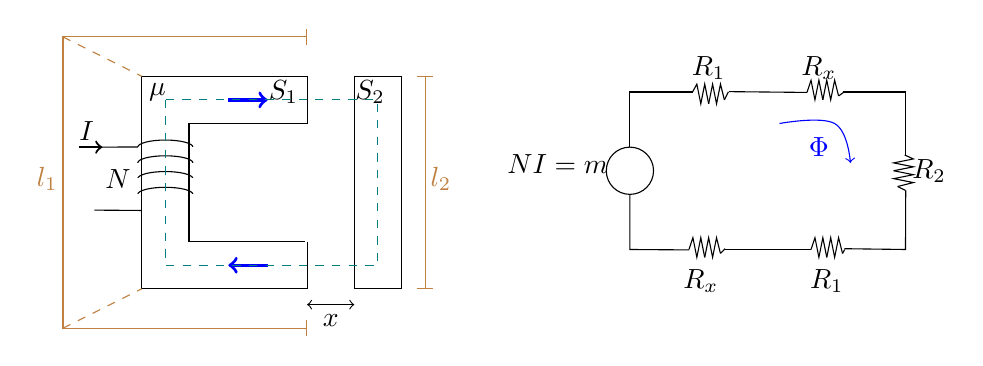
\begin{tikzpicture}

%el Relé
\draw  (-0.4,0.3) ellipse (0.35 and 0.09);
\draw [fill, white] (-0.8,0.3) rectangle (-0.0306,0.0956);
\draw  (-0.4,0.1) ellipse (0.35 and 0.09);
\draw [fill, white] (-0.7662,0.0912) rectangle (-0.0462,-0.1062);
\draw  (-0.4,-0.1) ellipse (0.35 and 0.09);
\draw [fill, white] (-0.7606,-0.1006) rectangle (-0.005,-0.2962);
\draw  (-0.4,-0.3) ellipse (0.35 and 0.09);
\draw [fill, white] (-0.8,-0.3) rectangle (0,-0.5);
\draw  (-0.7,1.2) node (v4) {} rectangle (2,-1.5);
\draw  (-0.1,0.6) rectangle (1.4,-0.9) node (v2) {};

\draw (-1.3,0.3) -- (-0.7474,0.3019);
\draw (-1.3,-0.5) -- (-0.7036,-0.5043);
\draw [thick,->] (-1.5,0.3) -- (-1.2,0.3);
\node at (-1.4,0.5) {$I$};
\node at (-1,-0.1) {$N$};
\draw [very thick, ->, blue] (0.4,0.9) -- (0.9,0.9);
\draw [very thick, <-, blue] (0.4,-1.2) -- (0.9,-1.2);
\draw (1.4,0.6) node (v1) {};
\draw [very thick, white](v1.center) -- (v2.center);
\draw   [fill, white](1.4,1.3) rectangle (2.2,-1.7);
\draw (1.4,1.2) -- (v1.center);
\draw (v2.center) -- (1.4,-1.5);
\draw  (2,1.2) rectangle (2.6,-1.5);
\draw  [dashed, teal](-0.4,0.9) rectangle (2.3,-1.2);
\draw [|-|, thin, brown](1.4,1.7) -- (-1.7,1.7) node (v3) {} -- (-1.7,-2) node (v5) {} -- (1.4,-2);
\node at (-1.9,-0.1) [brown]{$l_1$};
\node at (-0.5,1) {$\mu$};
\draw [|-|, thin, brown](2.9,1.2) -- (2.9,-1.5);
\node at (3.1,-0.1)  [brown]{$l_2$};
\draw [dashed, brown](v3.center) -- (v4.center);
\draw  [dashed, brown](v5.center) -- (-0.7,-1.5);
\node at (2.2,1) {$S_2$};
\node at (1.1,1) {$S_1$};


%circuito equivalente

\draw [scale=0.5] (17.98,0.4) -- (18.2,0.3) -- (17.7,0.2) -- (18.2,0.1) -- (17.7,0);
\draw [scale=0.5](17.7,0) -- (18.2,-0.1) -- (17.7,-0.2) -- (18.2,-0.3) -- (17.8,-0.4);
\draw [scale=0.5](17.8,-0.4) -- (18,-0.5);

\draw [scale=0.5, rotate=90] (-2,-15.6) -- (-1.7,-15.7) -- (-2.2,-15.8) -- (-1.7,-15.9) -- (-2.2,-16);
\draw [scale=0.5, rotate=90](-2.2,-16) -- (-1.7,-16.1) -- (-2.2,-16.2) -- (-1.7,-16.3) -- (-2.1,-16.4);
\draw [scale=0.5, rotate=90](-2.1,-16.4) -- (-2.0009,-16.4557);

\draw [scale=0.5, rotate=90] (-2,-12.5) -- (-1.7,-12.6) -- (-2.2,-12.7) -- (-1.7,-12.8) -- (-2.2,-12.9);
\draw [scale=0.5, rotate=90](-2.2,-12.9) -- (-1.7,-13) -- (-2.2,-13.1) -- (-1.7,-13.2) -- (-2.1,-13.3);
\draw [scale=0.5, rotate=90](-2.1,-13.3) -- (-1.9807,-13.4155);

\draw [scale=0.5, rotate=90] (2.0093,-12.5955) -- (2.2,-12.7) -- (1.7,-12.8) -- (2.2,-12.9) -- (1.7,-13);
\draw [scale=0.5, rotate=90](1.7,-13) -- (2.2,-13.1) -- (1.7,-13.2) -- (2.2,-13.3) -- (1.8,-13.4);
\draw [scale=0.5, rotate=90](1.8,-13.4) -- (2,-13.5);

\draw [scale=0.5, rotate=90] (2,-15.5) -- (2.3,-15.6) -- (1.8,-15.7) -- (2.3,-15.8) -- (1.8,-15.9);
\draw [scale=0.5, rotate=90](1.8,-15.9) -- (2.3,-16) -- (1.8,-16.1) -- (2.3,-16.2) -- (1.9,-16.3);
\draw [scale=0.5, rotate=90](1.9,-16.3) -- (1.9893,-16.4255);

\draw  (5.5,0) circle (0.3);
\draw (5.5,0.3) -- (5.5,1) -- (6.3,1);
\draw (6.7577,1.0047) -- (7.7527,0.9947);
\draw (8.2,1) -- (9,1) -- (9,0.2);
\draw (9.0027,-0.2503) -- (9,-1) -- (8.225,-0.99);
\draw (7.8,-1) -- (6.7,-1);
\draw (5.5,-0.3) -- (5.5,-1) -- (6.2527,-1.0053);
\node at (4.5838,0.0849) {$NI=\mathfrak{m}$};

\draw [->, blue] plot[smooth, tension=.7] coordinates {(7.4,0.6) (8.1,0.6) (8.3,0.1)};
\node at (7.9,0.3)[blue] {$\Phi$};
\draw [<->] (1.4,-1.7) -- (2,-1.7) node [midway,below] {$x$};
\node at (6.5,1.3) {$\mathscr{R}_1$};
\node at (7.9,1.3) {$\mathscr{R}_x$};
\node at (9.3,0) {$\mathscr{R}_2$};
\node at (6.4,-1.4) {$\mathscr{R}_x$};
\node at (8,-1.4) {$\mathscr{R}_1$};
\end{tikzpicture}